\documentclass[landscape]{foils} 
\newif\ifpdf
\ifx\pdfoutput\undefined
\pdffalse % we are not running PDFLaTeX
\else
\pdfoutput=1 % we are running PDFLaTeX
\pdftrue
\fi

\ifpdf
\usepackage[pdftex]{graphicx}
\else
\usepackage{graphicx}
\fi

\ifpdf
\DeclareGraphicsExtensions{.pdf, .jpg, .tif, .png}
\else
\DeclareGraphicsExtensions{.eps, .jpg}
\fi

%\usepackage{pslatex}
\usepackage{tabularx,dcolumn, graphicx, amsfonts,amsmath}  
\usepackage[sectionbib]{natbib}
\bibliographystyle{apalike}
\usepackage{picinpar}
\usepackage{multirow}
\usepackage{rotating}
\usepackage{paralist} %compactenum
\setlength{\voffset}{-0.5in}
%\setlength{\hoffset}{-0.5in}
%\setlength{\textwidth}{10.5in}
\setlength{\textheight}{7in}
\setlength{\parindent}{0pt}
%\pagestyle{empty}
%\renewcommand{\baselinestretch}{2.0}
\DeclareMathSymbol{\expect}{\mathalpha}{AMSb}{'105}
\def\p{\rm p}
\def\pp{\rm P}
% this are commands that come with the color package
\usepackage{color}
\usepackage{fancyhdr}


\pagestyle{empty}
%define colors
\definecolor{mediumblue}{rgb}{0.0509,0.35,0.568}
\definecolor{blue}{rgb}{0.0109,0.15,0.468}
\definecolor{black}{rgb}{0.04,0.06,0.2}
\definecolor{darkblue}{rgb}{0.03,0.1,0.2}
\definecolor{darkgreen}{rgb}{0.03,0.5,0.2}
\definecolor{lightblue}{rgb}{0.85,0.9333,0.95}
\definecolor{lightblue2}{rgb}{0.270588, 0.45098, 0.701961}
\definecolor{white}{rgb}{1.0,1.0,1.0}
\definecolor{yellow}{rgb}{0.961,0.972,0.047}
\definecolor{red}{rgb}{0.9,0.1,0.1}
\definecolor{orange}{rgb}{1.0,0.4,0.0}
\definecolor{grey}{rgb}{0.5,0.5,0.5}
\definecolor{violet}{rgb}{0.619608, 0.286275, 0.631373}
\definecolor{mybackgroundcolor}{rgb}{1.0,1.0,1.0}

%\definecolor{light}{rgb}{.5,0.5,0.0}
\definecolor{light}{rgb}{.3,0.3,0.3}

% sets backgroundcolor for whole document 
\pagecolor{mybackgroundcolor}
% sets text color
%\color{black}
% see below for an example how to change just a few words
% using \textcolor{color}{text}

\font \courier=pcrb scaled 2000
\newcommand{\notetoself}[1]{{\textsf{\textsc{\color{red} #1}}}\\}

\newcommand{\answer}[1]{{\sf \color{red} #1}}

\usepackage{pdfpages}

\newcommand{\section}{\secdef \newsection\newsection}
%\renewcommand{\labelitemi}{\includegraphics[width=5mm]{images/bullet.pdf}}
\newcommand{\newsection}[1]{%
{
	\par\flushleft\large\sf\bfseries \vskip -2cm #1\\\rule[0.7\baselineskip]{\textwidth}{0.5mm}\par}}

\newcommand{\subsection}{\secdef \test\test}
\newcommand{\test}[1]{%
	{\par\flushleft\normalsize\sf\bfseries #1: }}
\newcommand{\M}{\mathcal{M}}
\newcommand{\prob}{{\rm Prob~}}
\def\showy#1{{\normalsize\sf\bfseries #1}}
\def\donotuse#1{}

\newcommand{\entrylabel}[1]{\mbox{#1}\hfil}
\newenvironment{entry}
	{\begin{list}{}%
		{\renewcommand{\makelabel}{\entrylabel}%
		\setlength{\labelwidth}{35pt}%
		\setlength{\leftmargin}{\labelwidth+\labelsep}%
	}%
	{\end{list}}}

\newcommand{\poltext}{{\copyright\ 2002--2010 by Paul O. Lewis -- Modified by  Mark Holder with permission from Paul Lewis}}

\newcommand{\pol}{{\footnotesize \poltext}}
\newcommand{\myBackground}{\begin{picture}(0,0)(0,0)  \put(-40,-70){\makebox(0,0)[l]{\includegraphics[width=33cm]{images/baby_blue.jpg}}} \end{picture}}
\newcommand{\myFooter}{}
%\begin{picture}(0,0)(0,0)
%	\put(0,-185){\pol}
%\end{picture}}
\newcommand{\myNewSlide}{\newpage\myFooter} % \myBackground}

\usepackage{url}
\usepackage{hyperref}
\hypersetup{backref,  linkcolor=blue, citecolor=black, colorlinks=true, hyperindex=true}

\usepackage{pdfpages}
\usepackage{bm}
\usepackage{ifsym}

\begin{document}

\myNewSlide
\huge 
Thanks to Paul Lewis, Joe Felsenstein, and Peter Beerli for slides.

\myNewSlide
\section*{Reasons phylogenetic inference might be wrong}
\Large
\begin{compactenum}
	\item Our data might be wrong (``garbage in garbage out'')
	\item {\em Systematic error} -- our inference method might not be sophisticated enough
	\item \underline{{\em Random error}} -- We might not have enough data, so we are misled by sampling error.
\end{compactenum}

(or it could be some combination of these).

{Focus of this evenging: How confident can we be in the trees/splits inferred by ML?}

\myNewSlide
\begin{compactenum}
	\item Bootstrapping to assess repeatability;
	\item Putting $P$-values on trees:
	\begin{compactitem}
		\item KH Test, SH Test
		\item aLRT, aBayes,
		\item parametric bootstrapping,
		\item 1 - BP,
		\item Discussion of the theory underlying this plethora of testing methods, and the history of the debates around bootstrapping in phylogenetics,
		\item AU,
		\item aBP
	\end{compactitem}
	\item brief lab on how to use {\tt Seq-Gen} to conduct parametric bootstrapping.
\end{compactenum}


\myNewSlide
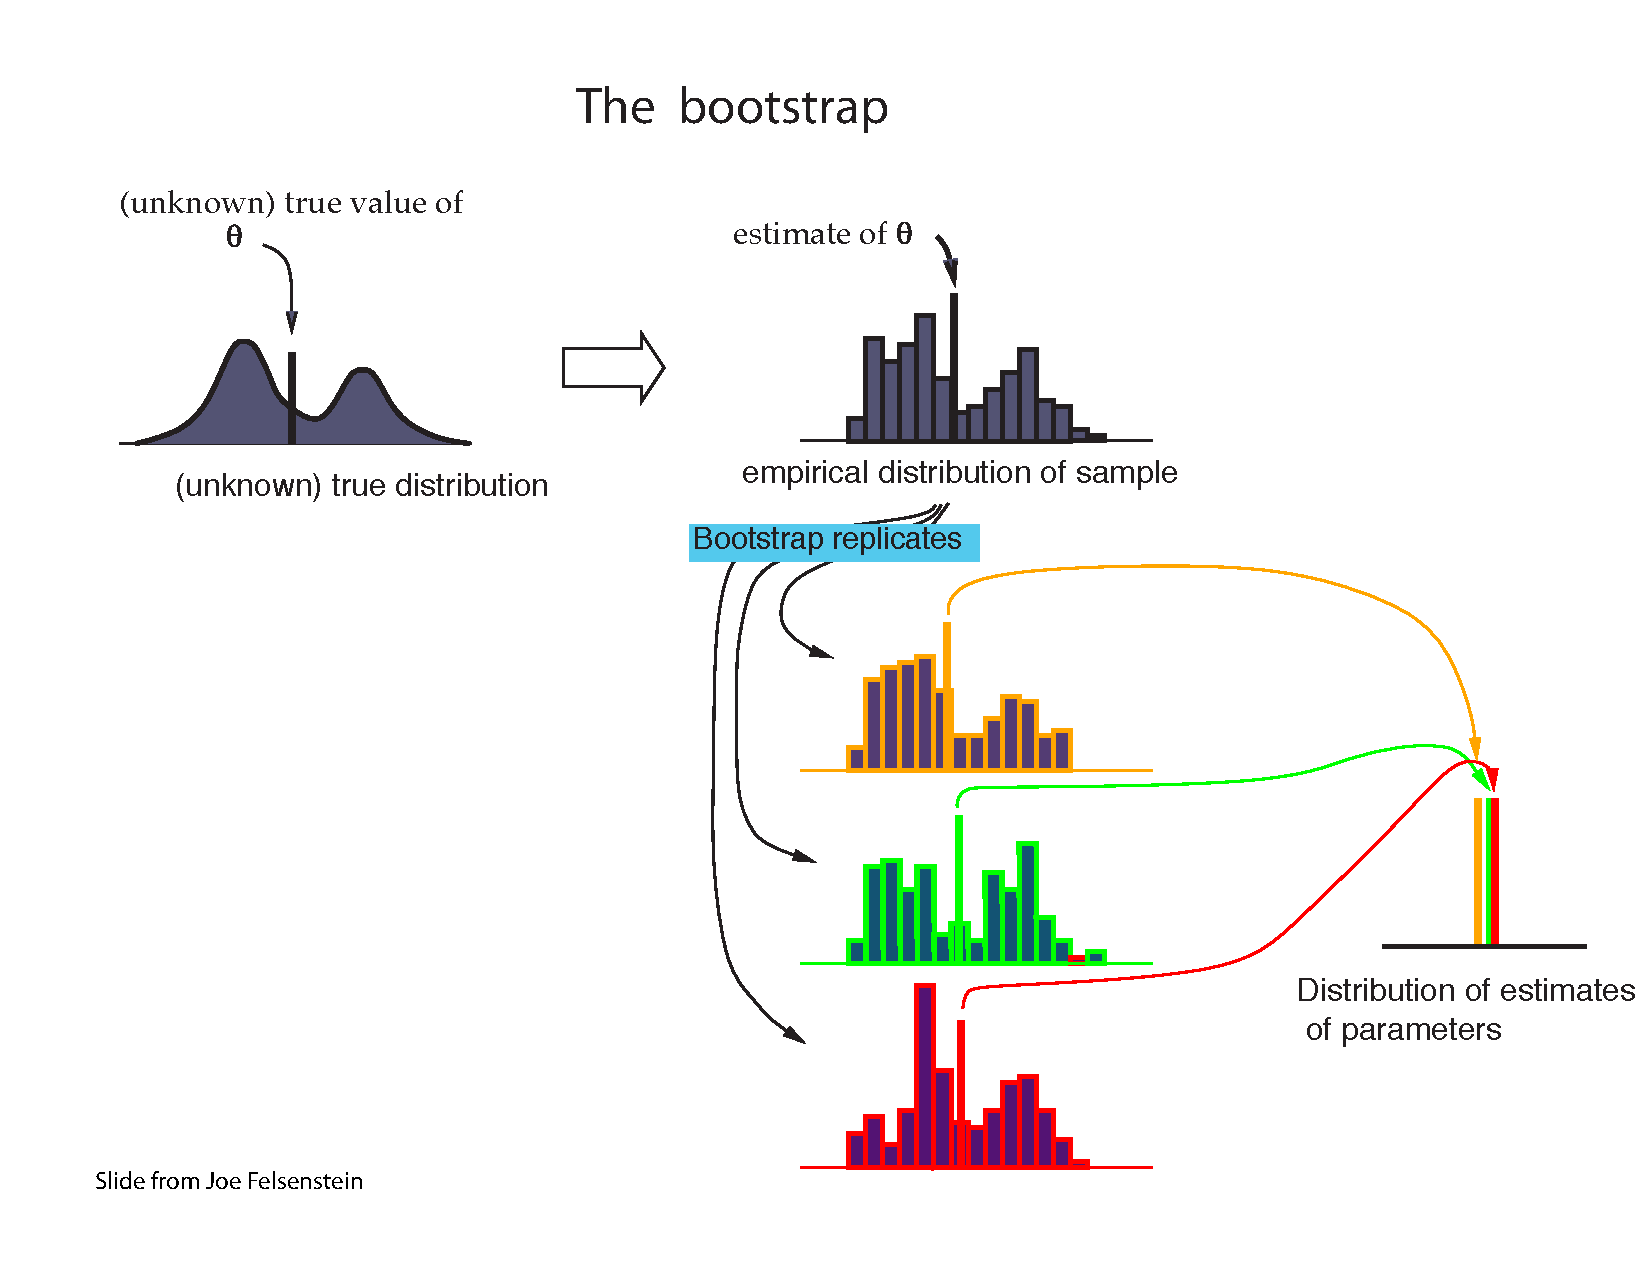
\includepdf[pages={1}]{../newimages/JoeFelsBootFig1.pdf} 

\myNewSlide
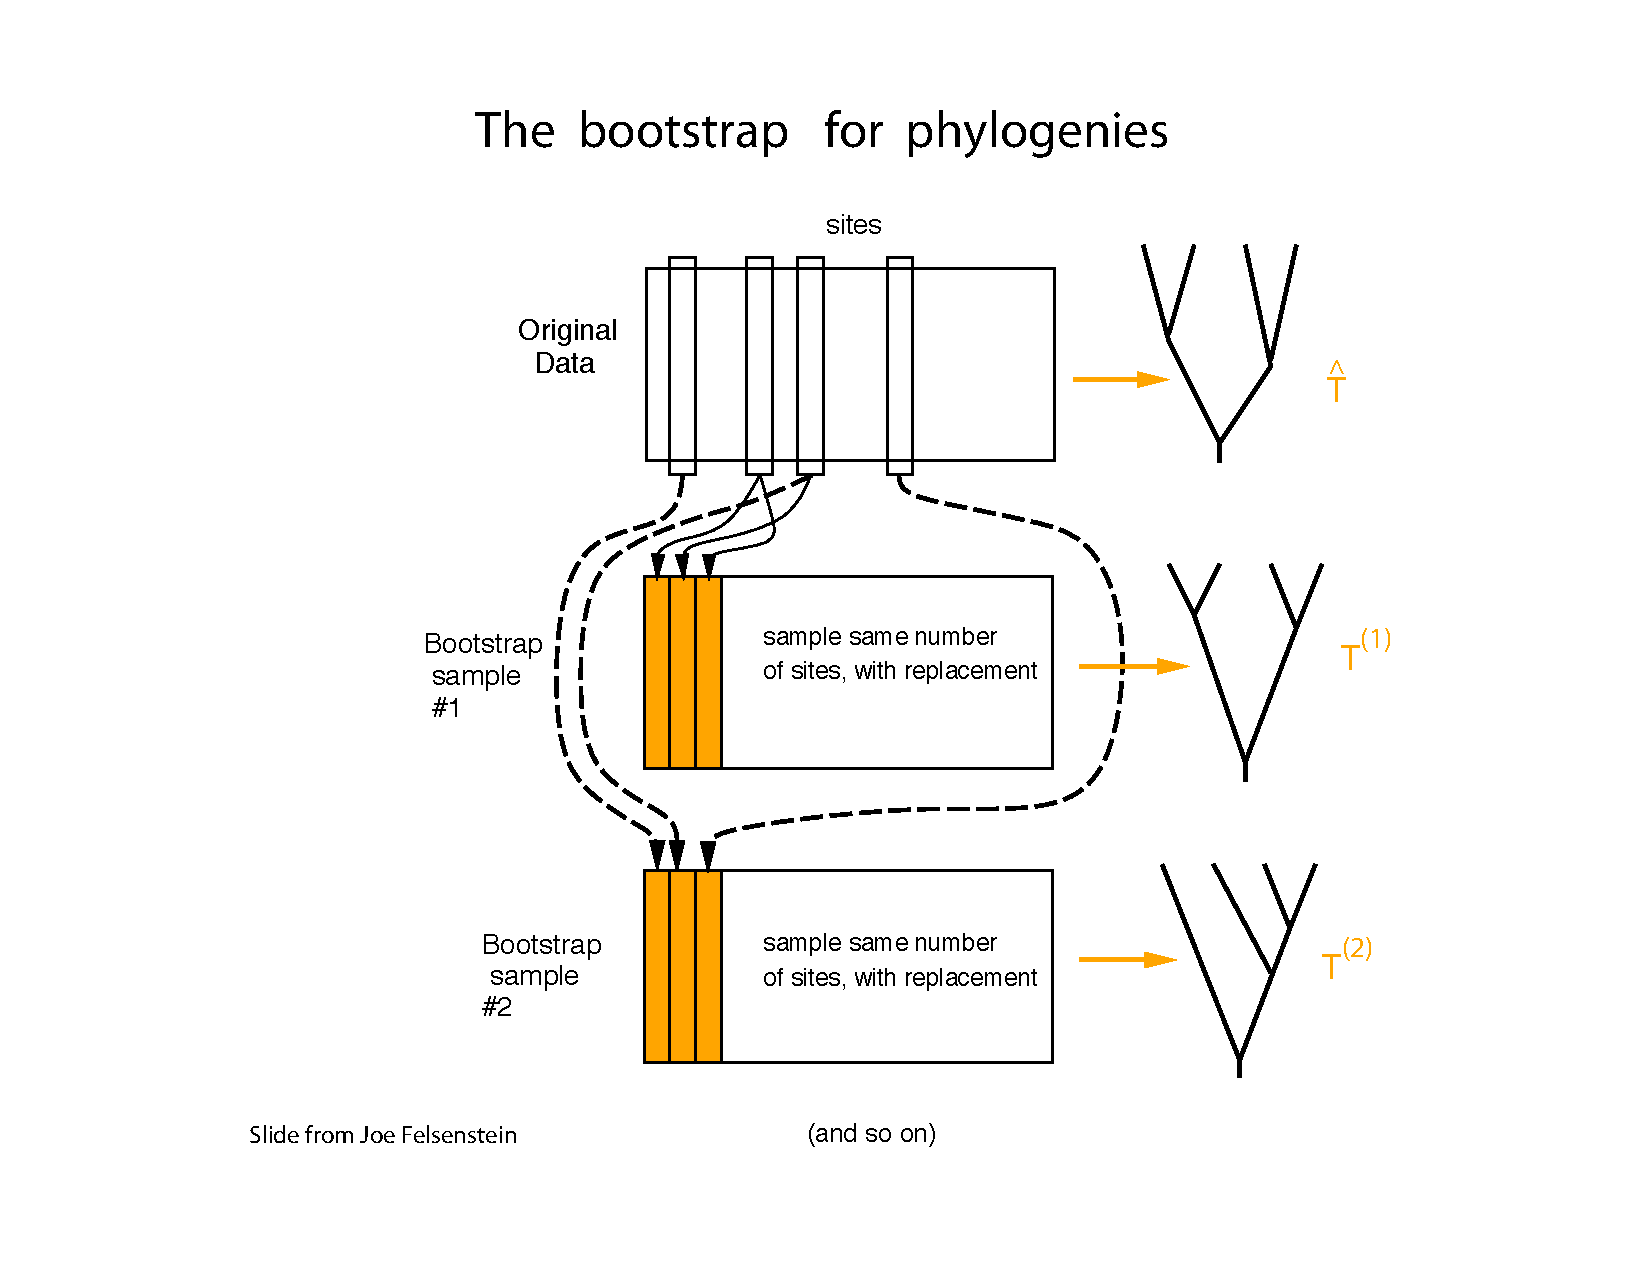
\includepdf[pages={1}]{../newimages/JoeFelsBootFig2.pdf} 

\myNewSlide
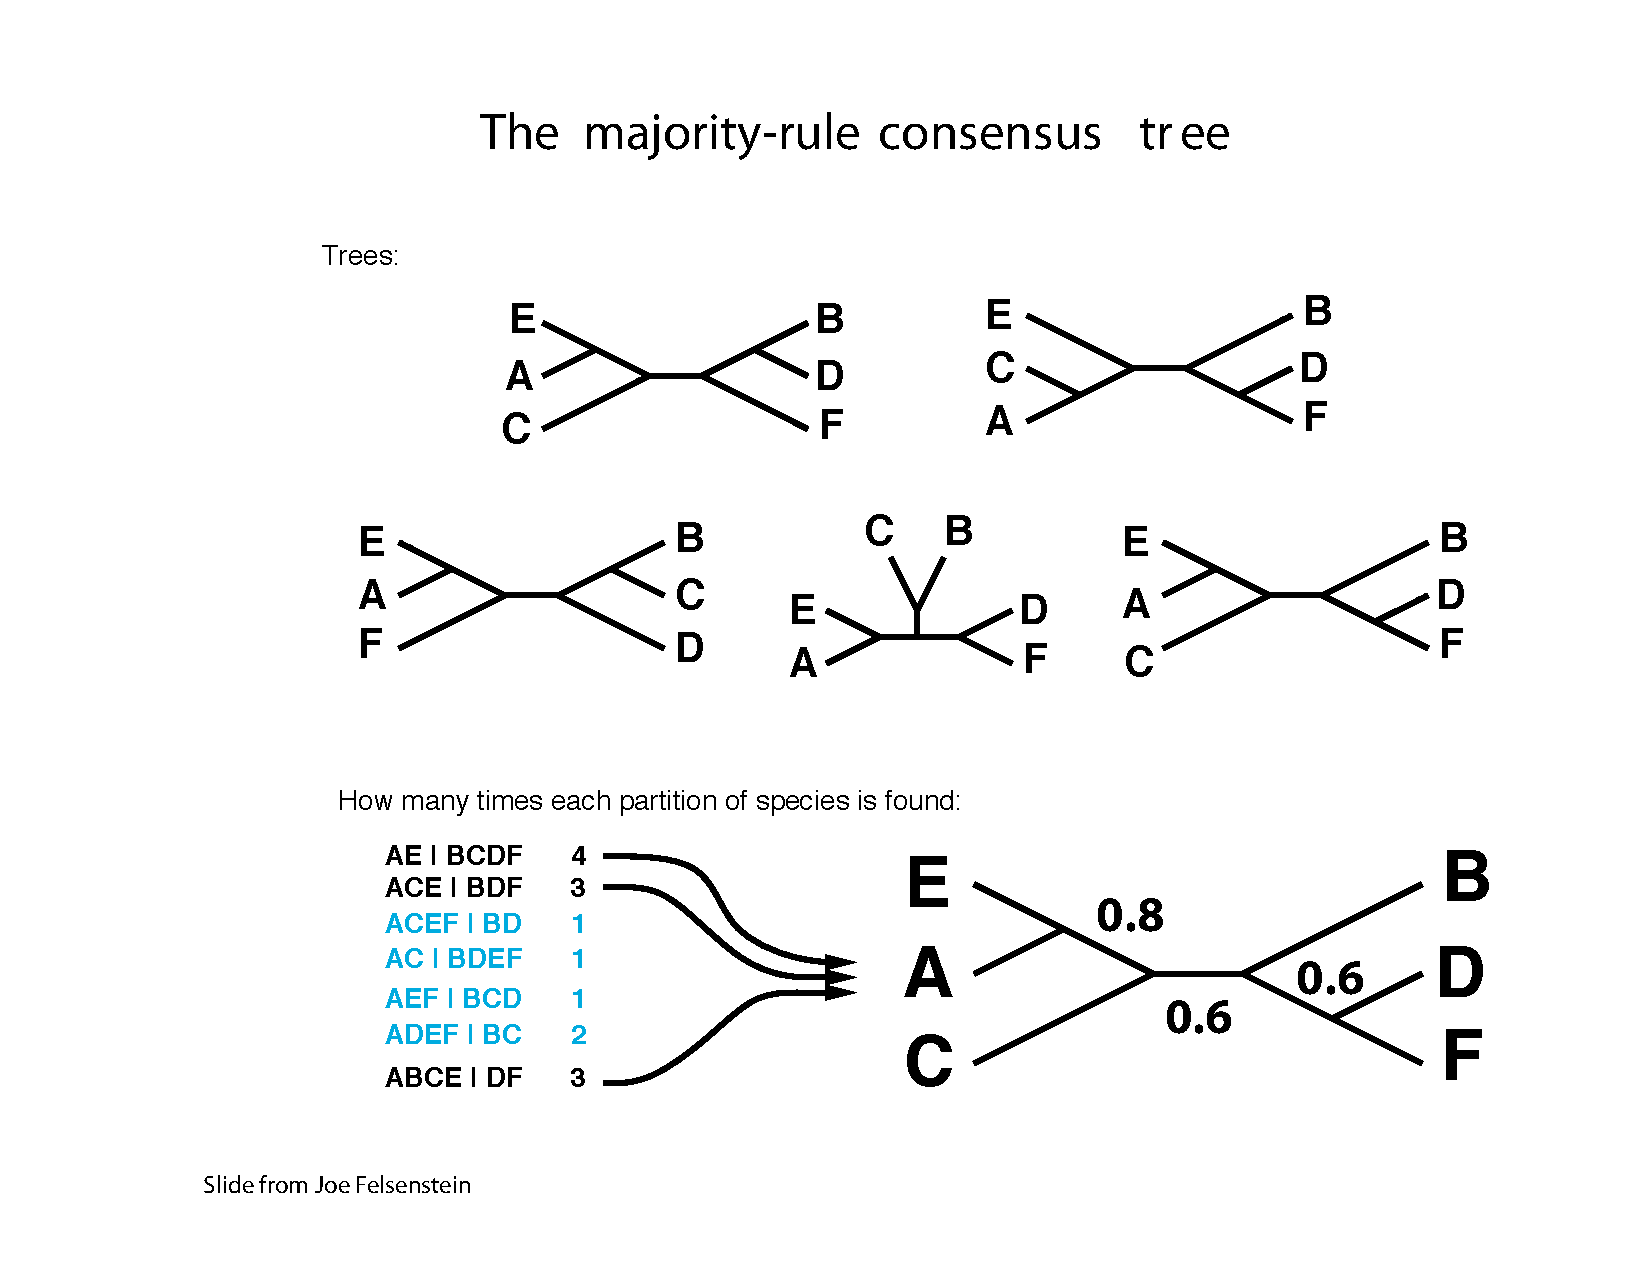
\includepdf[pages={1}]{../newimages/JoeFelsBootFig3.pdf} 
\myNewSlide
\begin{picture}(0,0)(0,0)
	  \put(0,-180){\makebox(0,0)[l]{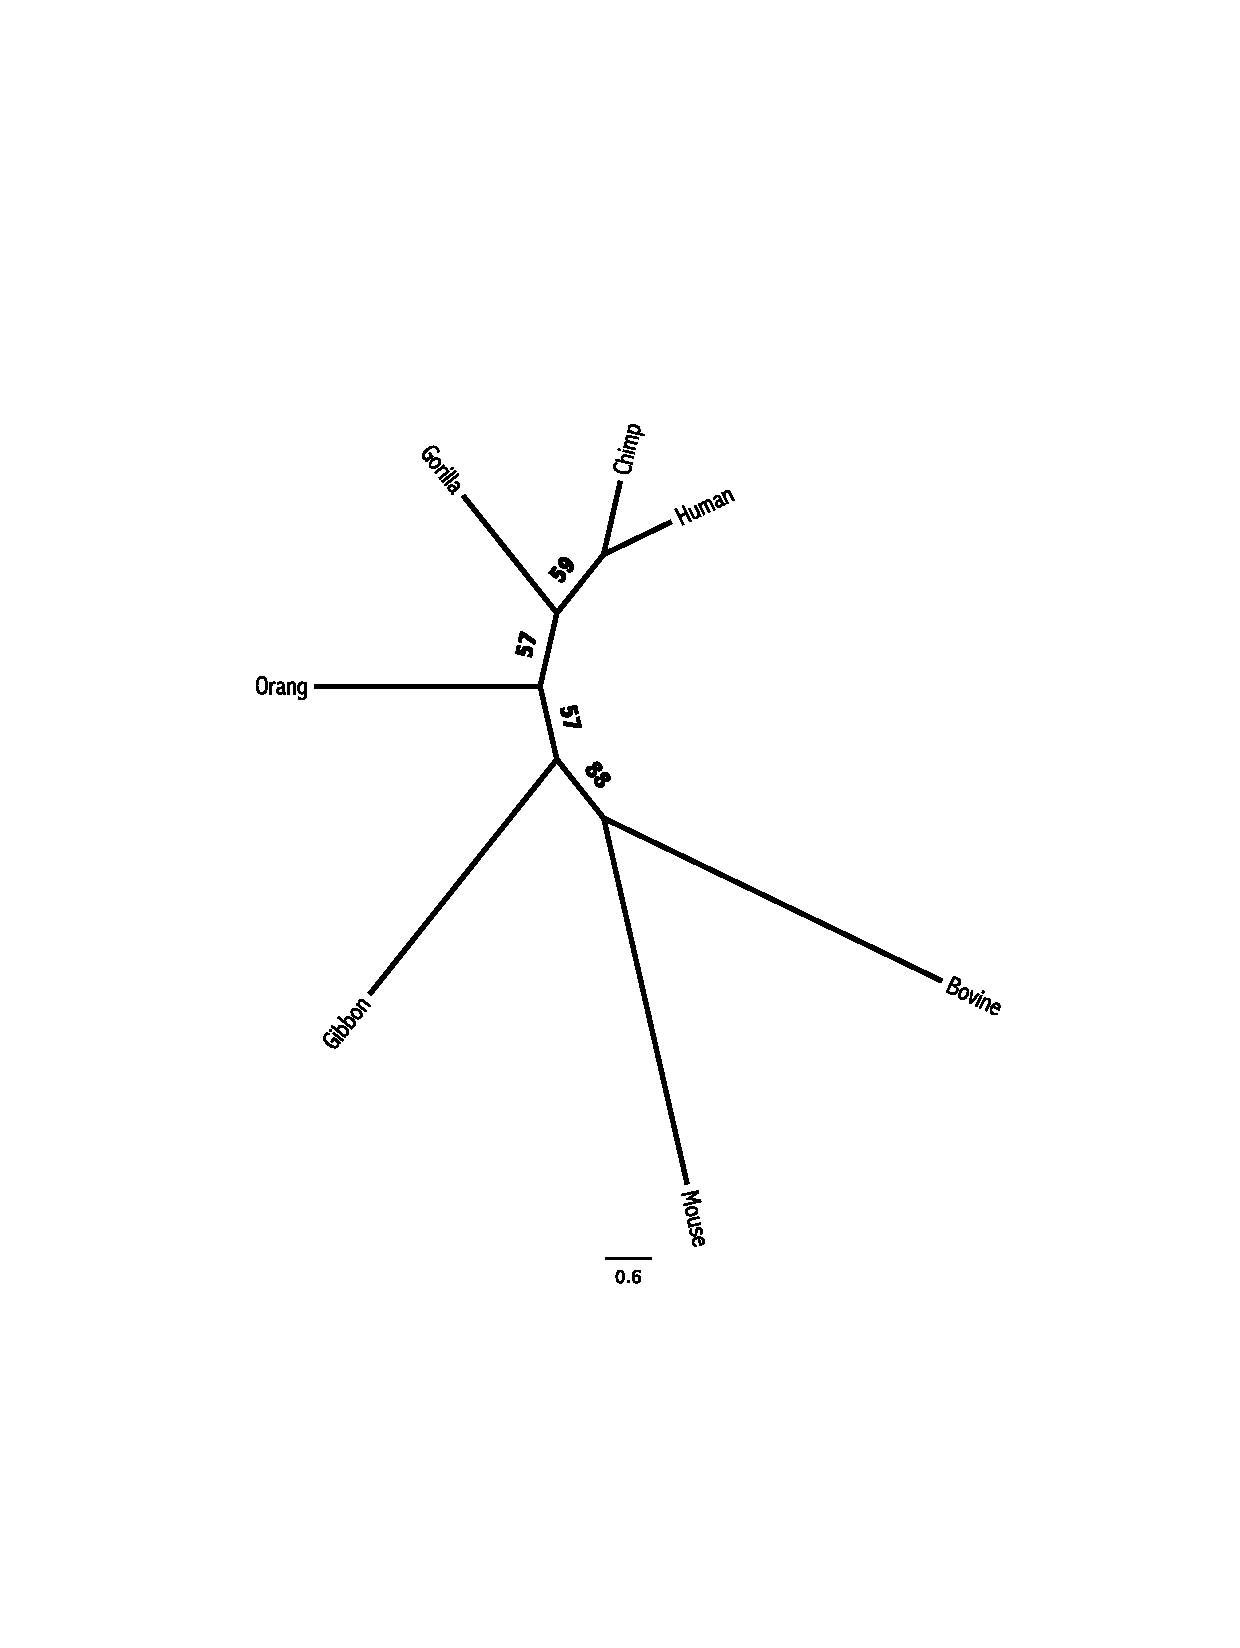
\includegraphics[scale=1.2]{../newimages/hasegawaBootFigTree.pdf}}}
	  \put(0,-350){\small From Hasegawa's analysis of 232 sites D-loop}
\end{picture}

\myNewSlide
\section*{Bootstrapping for branch support}
\large
\begin{itemize}
	\item ``Rogue'' taxa can lower support for many splits -- you do not have to use the majority-rule consensus tree to summarize bootstrap confidence statements.
	\item Less thorough searching is faster, but will usually artificially lower BP. However, \citet{AnisimovaGDDG2011} report that RAxML's rapid bootstrap algorithm may inflate bootstrap proportions).
\end{itemize}


\myNewSlide
\section*{Frequentist hypothesis testing: coin flipping example}
$N=100$ and $h=60$\\
Can we reject the hypothesis of a fair coin ($p_H = 0.5$)?

The ``recipe'' is:
\begin{compactenum}
	\item Formulate a null ($H_0$) and alternative ($H_A$) hypothesis.
	\item Choose an acceptable Type-I error rate.
	\item Choose a test statistic: $f_H$= fraction of heads in sample. $f_H=0.6$
	\item Identify the tail region of the test statistic - the values that conflict with $H_0$ at least a strongly as your observed data.
	\item Calculate the $P$-value: The probability of a test statistic value more extreme than $0.6$ arising {\em even if $H_0$  is true}.
	\item Reject $H_0$ if $P$-value is $\leq$ your Type I error rate.
\end{compactenum}

\myNewSlide
\begin{picture}(500,0)(0,0)
	  \put(0,-190){\makebox(0,0)[l]{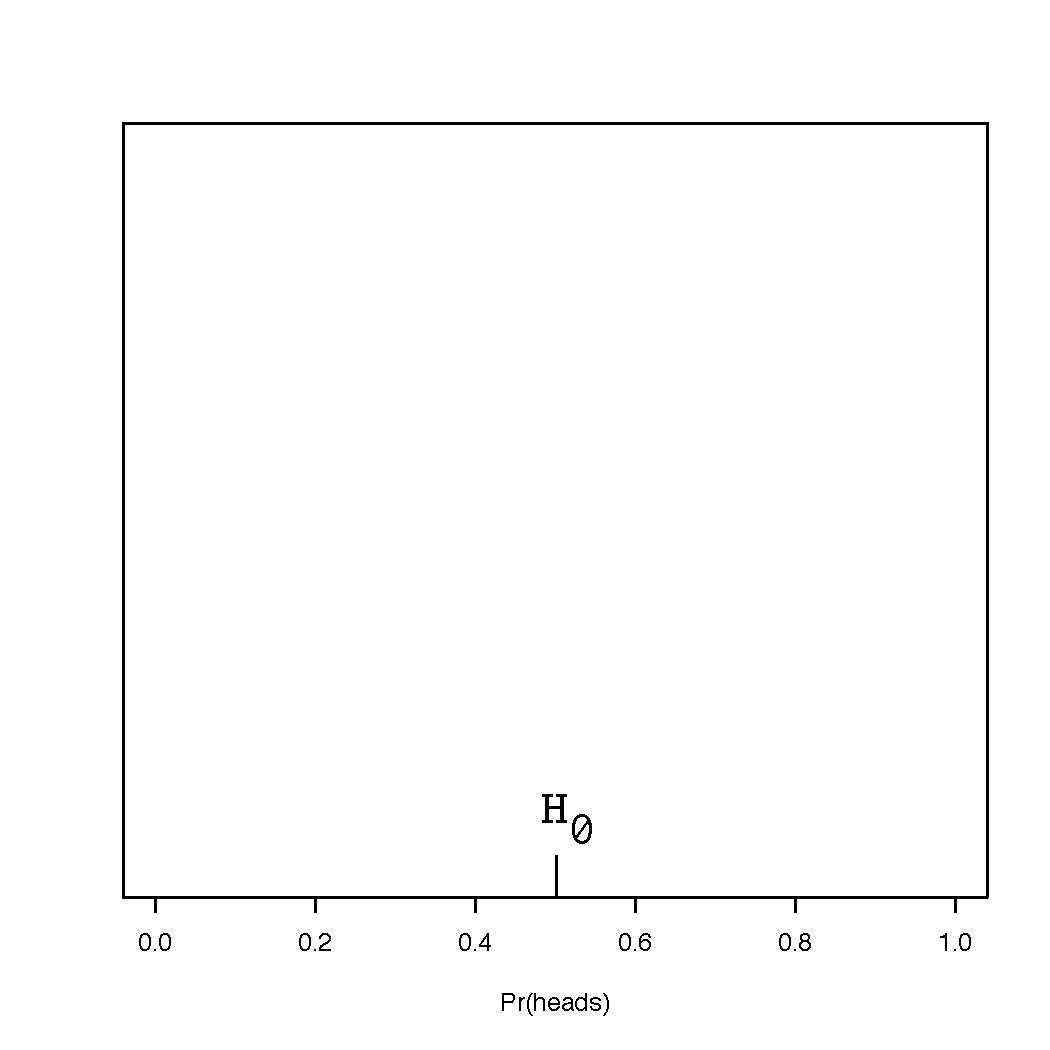
\includegraphics[scale=1.0]{../newimages/coin_axes.pdf}}}
\end{picture}

\myNewSlide
\begin{picture}(500,0)(0,0)
	  \put(0,-190){\makebox(0,0)[l]{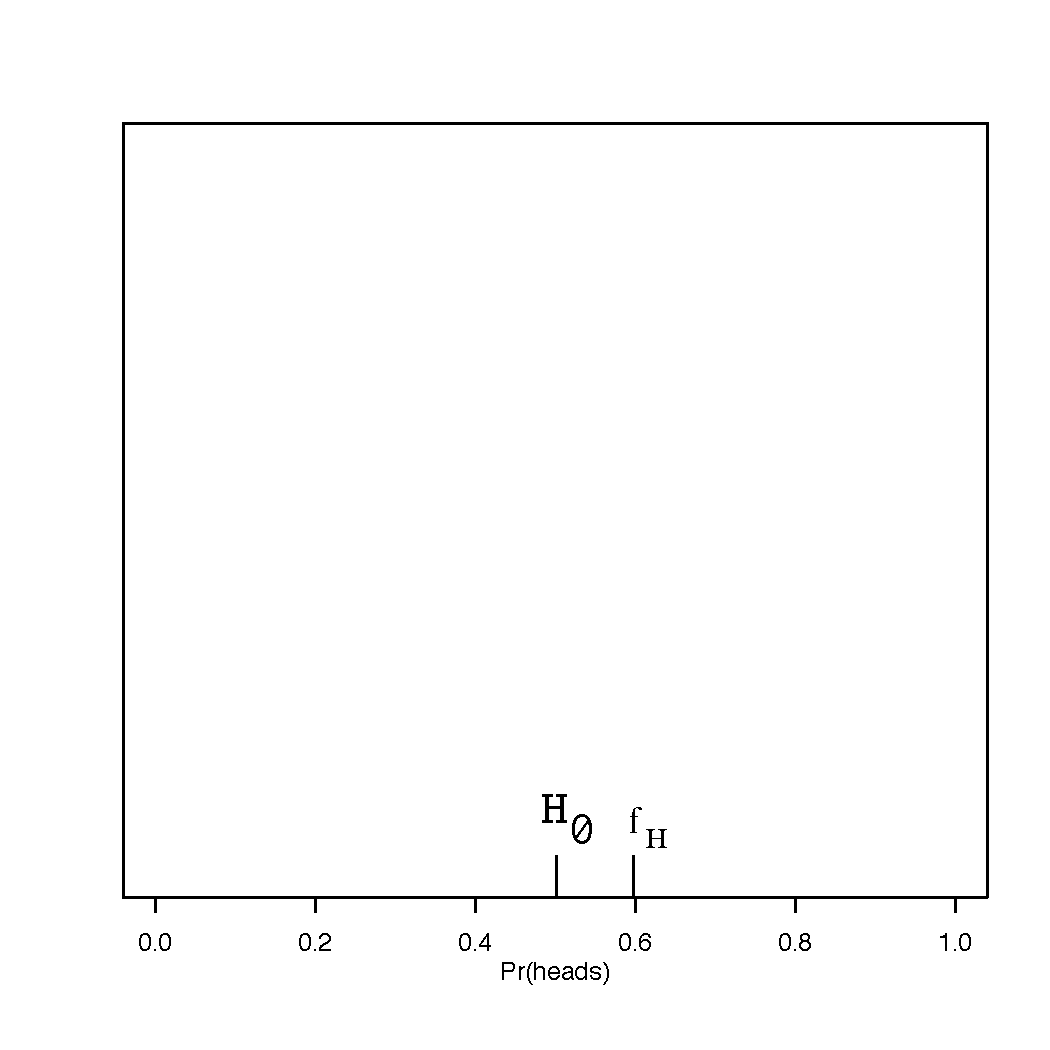
\includegraphics[scale=1.0]{../newimages/coin_axes_data.pdf}}}
\end{picture}

\myNewSlide
\begin{picture}(500,0)(0,0)
	  \put(0,-190){\makebox(0,0)[l]{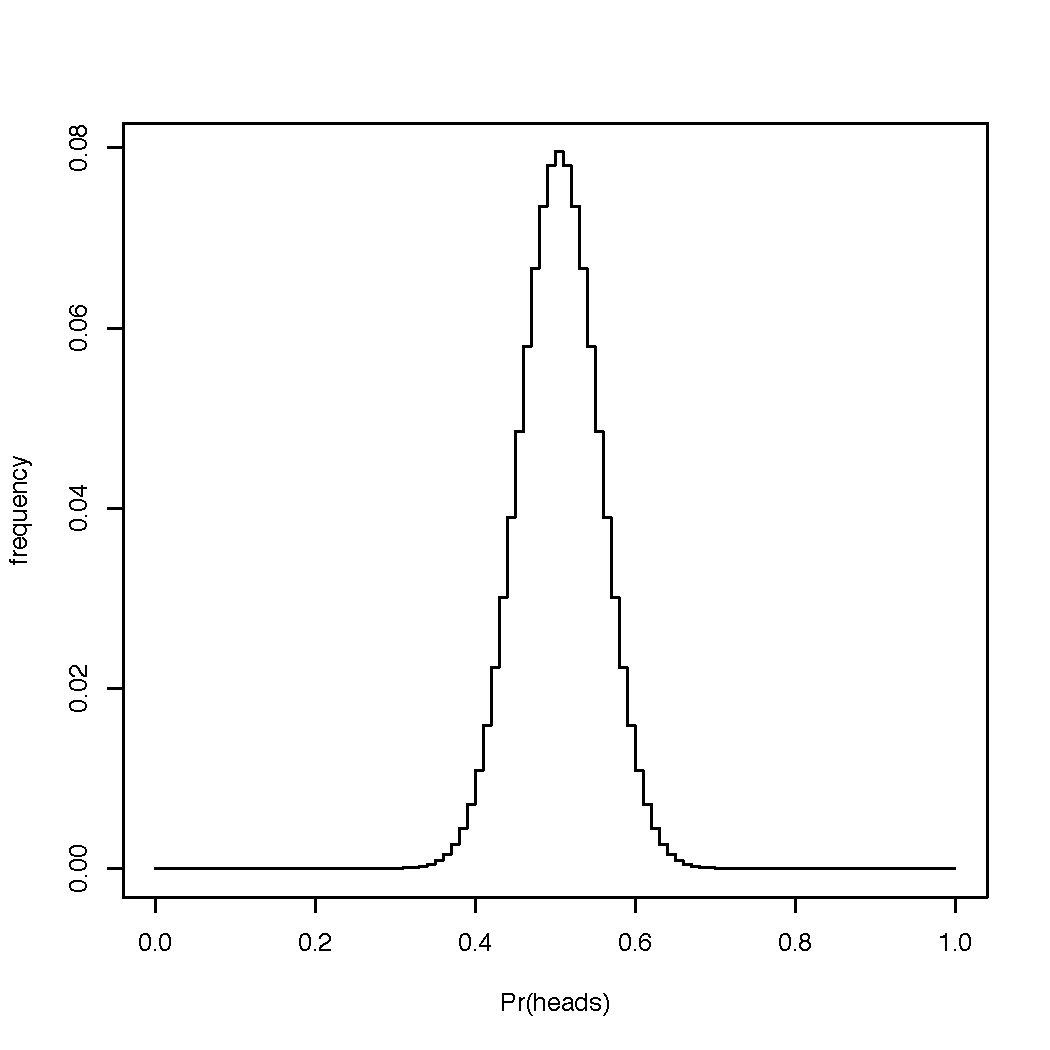
\includegraphics[scale=1.0]{../newimages/coin_wo_tails.pdf}}}
\end{picture}

\myNewSlide
\begin{picture}(500,0)(0,0)
	  \put(0,-190){\makebox(0,0)[l]{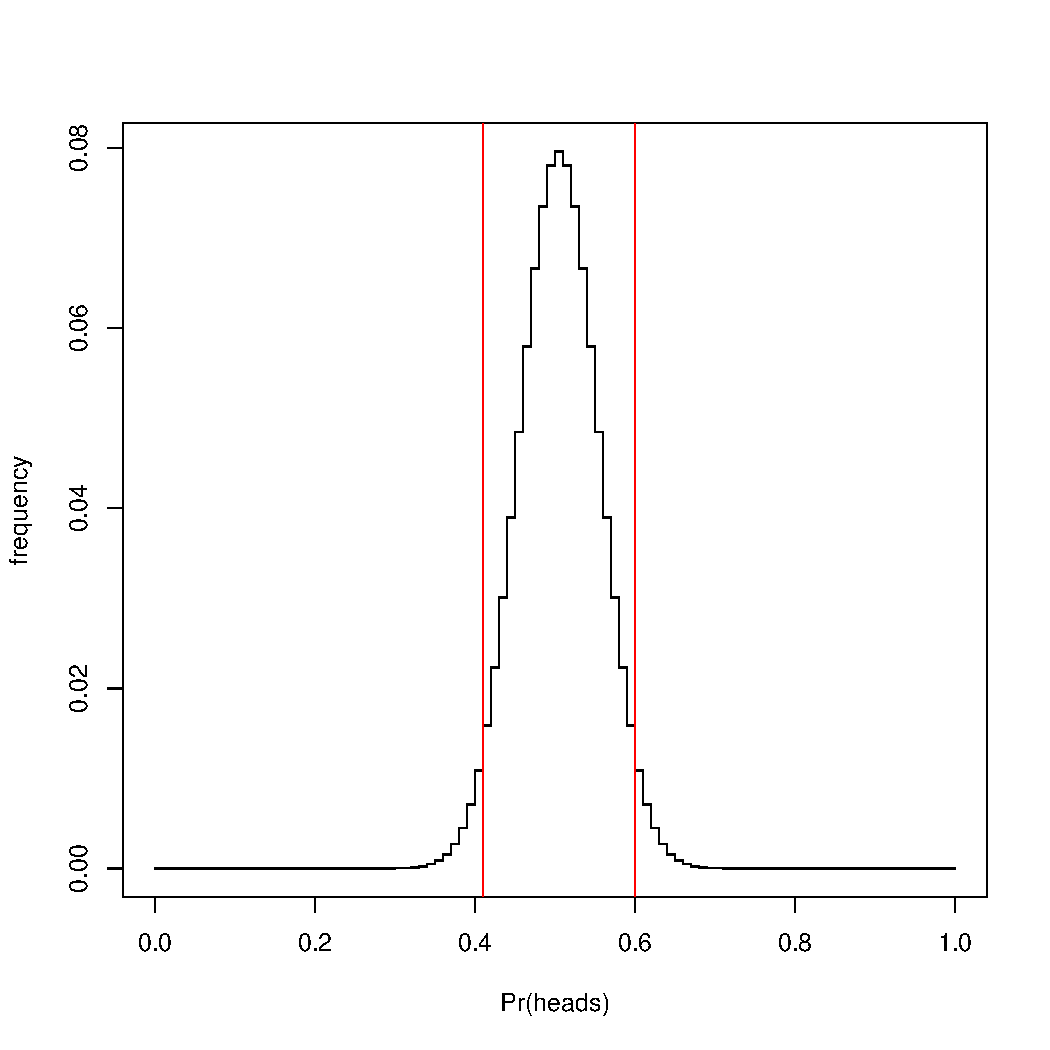
\includegraphics[scale=1.0]{../newimages/coin_w_tails.pdf}}}
	  \put(0,-450){$P$-value $\approx$ 0.056}
\end{picture}

\myNewSlide
Making similar plots for tree inference is hard.

Our parameter space is trees and branch lengths. Our data is a matrix of characters. It is hard to put these objects on the same plot.

We will see later, that we can visualize them both in a parameter space that describes how frequent different patterns of data are.


\myNewSlide
\section*{The simplest phylogenetic test would compare two trees}
\Large
Null: If we had no sampling error (infinite data) $T_1$ and $T_2$ would explain the data equally well. 

Test Statistic: $$\delta(T_1,T_2|X) = 2\left[\ln L(T_1|X) - \ln L(T_2|X)\right]$$

Expectation under null: $$\mathbb{E}_{H_0}\left[\delta(T_1,T_2|X)\right] = 0$$

\myNewSlide
\begin{picture}(500,0)(0,0)
	  \put(20,-20){\small Using 3000 sites of mtDNA sequence for 5 primates}
	  \put(20,-60){\normalsize $T_1$ is ((chimp, gorilla), human)}
	  \put(20,-100){\normalsize $T_2$ is ((chimp, human), gorilla)}
	  \put(-10,-385){\small$\delta(T_1,T_2|X)=-3.18$}
	  \put(300,-385){\small$\mathbb{E}(\delta)$}
	  \put(50,-150){\makebox(0,-190)[l]{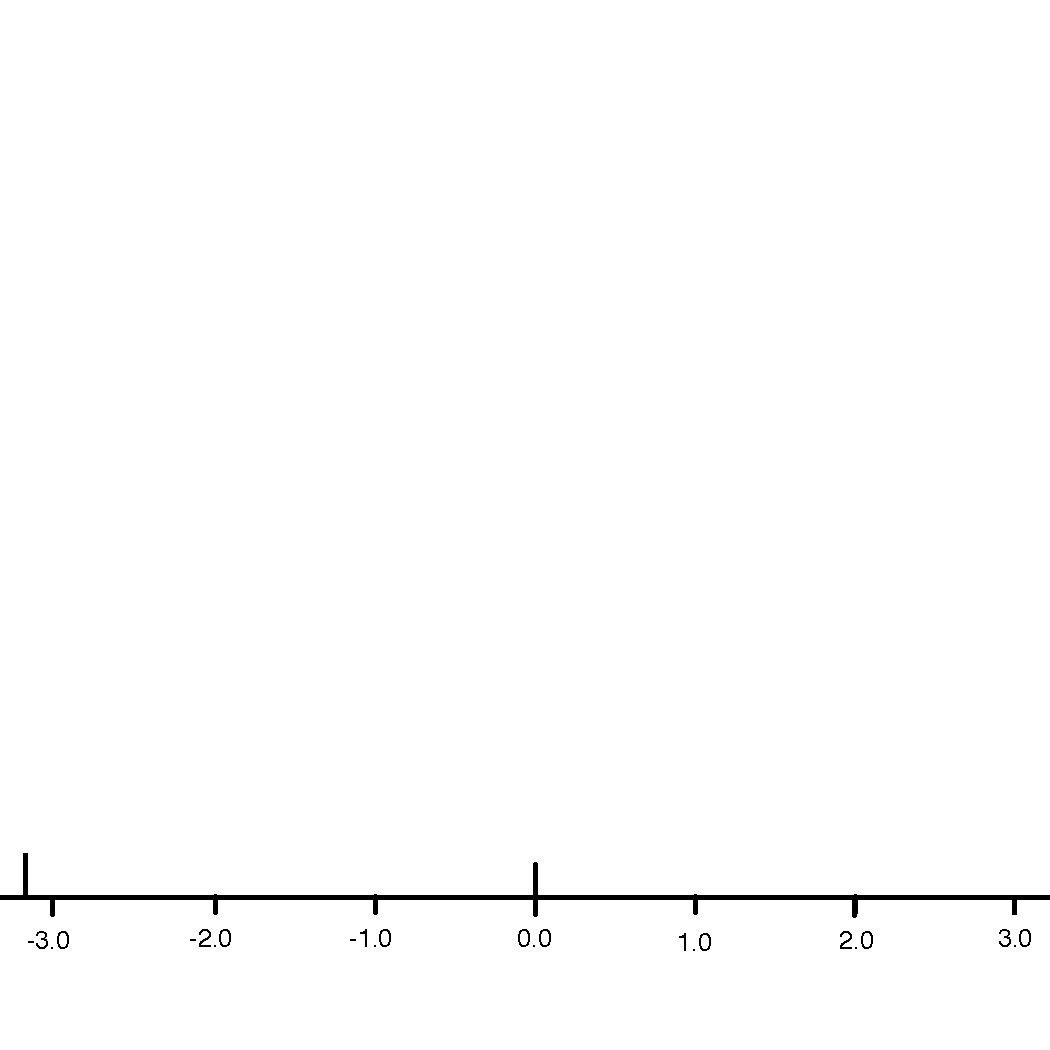
\includegraphics[scale=1.0]{../newimages/delta_axes.pdf}}}
	  \put(220,-480){$\delta(T_1,T_2|X) $}
\end{picture}




\myNewSlide

To get the $P$-value, we need to know the probability: $$\Pr\left(\big|\delta(T_1,T_2|X)\big| > 3.17 | H_0\mbox{ is true}\right) $$

\myNewSlide
\section*{KH Test}
\begin{compactenum}
	\item Examine at the difference in $\ln L$ for each site: $\delta(T_1,T_2|X_i)$ for site $i$.
	\item Note that the total difference is simply a sum:
		$$\delta(T_1,T_2|X) = \sum_{i=1}^M\delta(T_1,T_2|X_i)$$
	\item The variance of $\delta(T_1,T_2|X)$ will be a function of the variance in ``site'' $\delta(T_1,T_2|X_i)$ values.
\end{compactenum}



\myNewSlide
\begin{picture}(500,0)(0,0)
	  \put(0,-10){\large 2*difference in $\ln L$ for each site}
	  \put(280,-35){\large $\vdots$}
	  \put(20,-250){\makebox(0,0)[l]{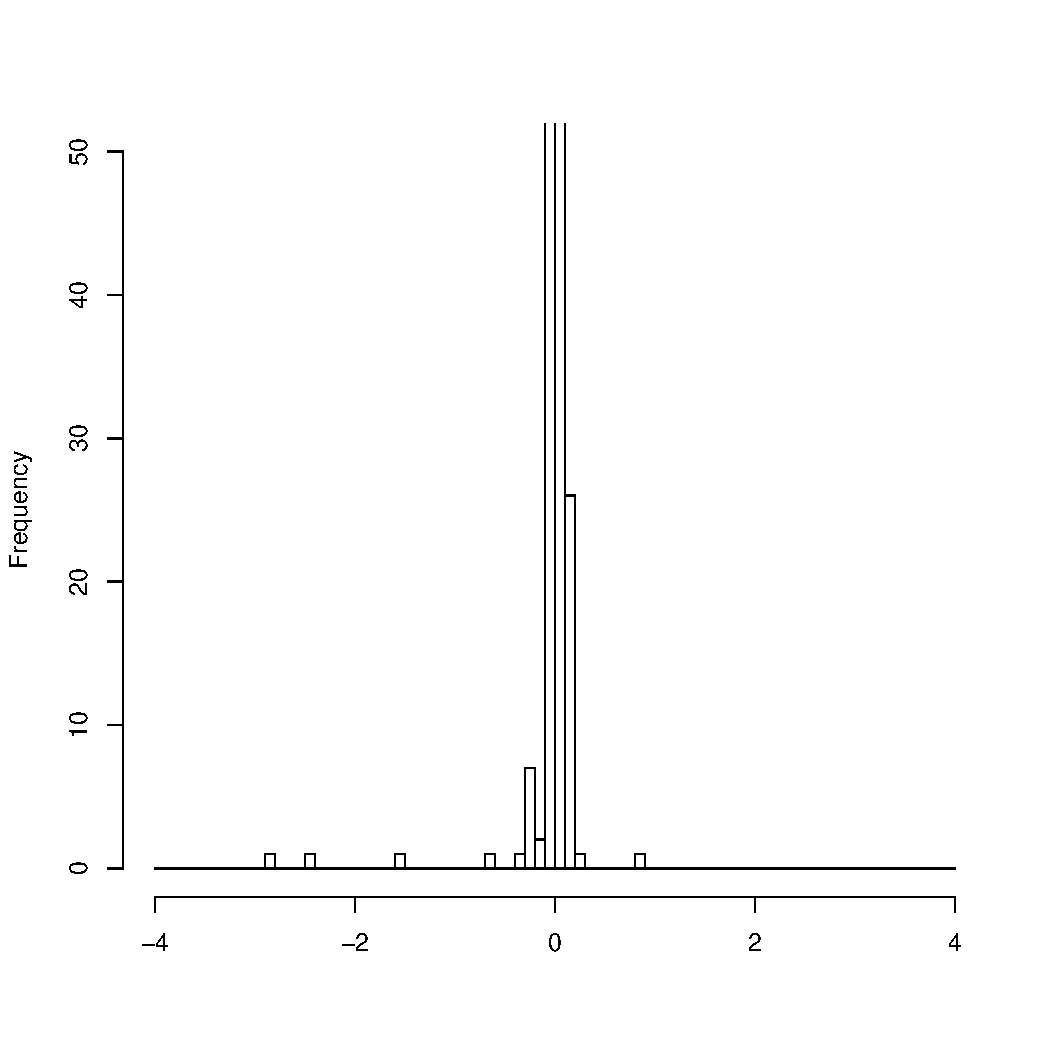
\includegraphics[scale=1.0]{../scripts/mtdna/d1-2hist.pdf}}}
	  \put(250,-490){\normalsize$\delta(T_1,T_2|x_i)$}
\end{picture}


\myNewSlide
\section*{KH Test - the variance of $\delta(T_1,T_2|X)$}
To get a sense of the variance of $\delta(T_1,T_2|X)$ we should expect because of sampling error, we could use:
\begin{compactenum}
	\item Assumptions of normality (by appealing to the Central Limit Theorem), or
	\item Bootstrapping to generate a cloud of pseudo-replicate $\delta(T_1,T_2|X^{\ast})$ values.
\end{compactenum}

\myNewSlide
\section*{RELL bootstrap}
If the MLE of the numerical parameters (including branch lengths) do not change much when we bootstrap we can simply resample the site $\ln L$ values and sum them.

This is called the RELL bootstrap \citep[][and Felsenstein]{KishinoMH1990}. It may not be very safe \citep[especially on large trees;][]{StamatakisHR2008}.
\myNewSlide
\begin{picture}(500,0)(0,0)
	  \put(0,-10){\large $\delta$ for many (RELL) bootstrapped replicates of the data}
	  \put(280,-35){\large $\vdots$}
	  \put(20,-250){\makebox(0,0)[l]{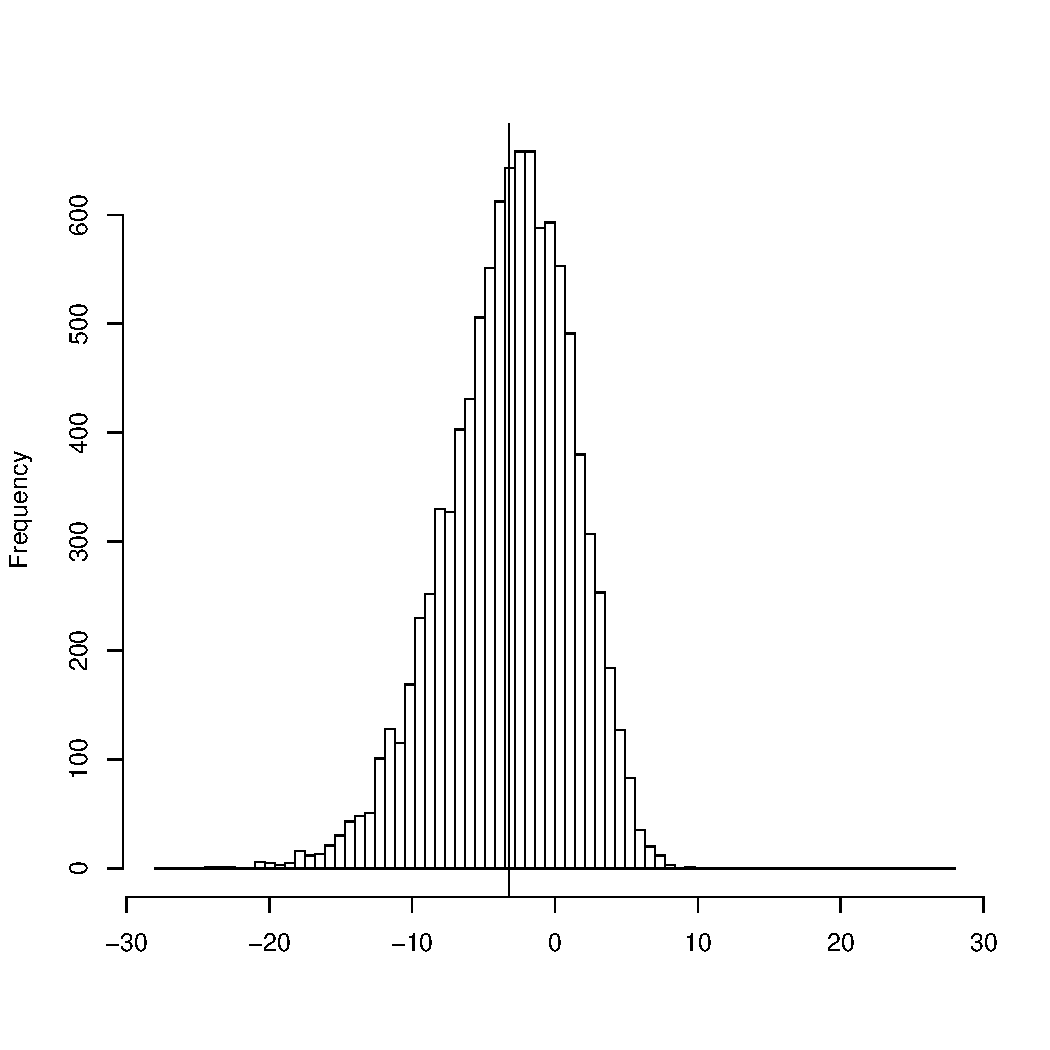
\includegraphics[scale=1.0]{../scripts/mtdna/uncentered1-2hist.pdf}}}
	  \put(250,-490){\normalsize$\delta(T_1,T_2|X^{\ast})$}
\end{picture}

\myNewSlide
\section*{KH Test - `centering'}
$H_0$ gives us the expected value: $$\mathbb{E}_{H_0}\left[\delta(T_1,T_2|X)\right] = 0$$
Bootstrapping gives us a reasonable guess of the variance under $H_0$

By substracting the mean of the bootstrapped $\delta(T_1,T_2|X^{\ast})$ values, we can create a null distribution.

For each of the $j$ bootstrap replicates, we treat $\delta(T_1,T_2|X^{\ast j}) - \bar\delta(T_1,T_2|X^{\ast})$  as draws from the null distribution.

\myNewSlide
CENTERED FIG

\myNewSlide
CENTERED FIG with $P$-value


\myNewSlide
\section*{What if start out with only one hypothesized tree, and we want to compare it to the ML tree?}
The KH Test is {\bf NOT} appropriate in this context \citep[see][for discussion of this point]{GoldmanAR2000}

{\bf Multiple Comparisons}: lots of trees increases the variance of $\delta(\hat{T},T_1|X)$\\

{\bf Selection bias}: Picking the ML tree to serve as one of the hypotheses invalidates the centering procedure of the KH test.

\myNewSlide
\section*{selection bias introduced by using the ML tree in your test}
Even when the $H_0$ is true, we do not expect $2\left[\ln L(\hat{T}) - \ln L(T_1)\right]= 0$

Imagine a competition in which a large number of equally skilled people compete, and you compare the score of one competitor against the highest scorer.

\myNewSlide
\section*{Shimodaira-Hasegawa proposed a test that deals the ``selection bias'' introduced by using the ML tree in your test}
You have to specify of a set of candidate trees - inclusion in this set {\bf must not} depend on the dataset to be analyzed.

The null hypothesis is that all members of the candidate set have the same expected score.

\myNewSlide
\section*{SH Test details}
\normalsize
\begin{compactitem}
	\item For each tree $T_i$ in the candidate set calculate $\delta(\hat{T}, T_i|X)$
	\item For each tree $T_i$, use $\bar{\ln L}(T_i|X^{\ast})$ to center the bootstrapped collection of log-likelihoods:
		$$c_i^{(j)} = {\ln L}(T_i|X^{\ast})-\bar{\ln L}(T_i|X^{\ast})$$
	\item For each replicate pick the highest value from the centered distributions (this mimics the selection bias): $$m^{(j)} = \max\left[c_i^{(j)}\right] \mbox{ over all } j$$
	\item The for each tree and replicate, you get a sample from the null $\delta_i^{(j)} = m^{(j)} - c_i^{(j)}$
	\item $P$-value for tree $T_i$ can be approximated by seeing where in the distribution of $\delta_i^{(j)}$ values it lies (the $P$-value is the proportion of sampled $\delta_i^{(j)} \geq \delta_i$
\end{compactitem}

\myNewSlide
\section*{SH test candidate set selection}
\large
\begin{compactitem}
	\item The candidate set should be all trees that you would have seriously entertained before seeing the data. 
	\item Using all trees is safe (though weakens the test, and is computationally demanding).
	\item Unfortunately, only considering a subset of trees for computational convenience can invalidate the test.
	\item If a tree has low $\ln L$ and low variance of site-log-likelihoods then it can probably be safely removed without affecting the $P$-values of other trees\footnote{Because such a tree would be unlikely to ever be the tree that is the determines the maximum diplacement from the centered value, $m^{(j)}$.}
\end{compactitem}
The test makes worst-case assumptions about the range of plausible $\ln L$ values. As a result the SH test is too conservative.

\myNewSlide
\large
\begin{picture}(500,0)(0,0)
	  \put(-200,-190){\makebox(0,0)[l]{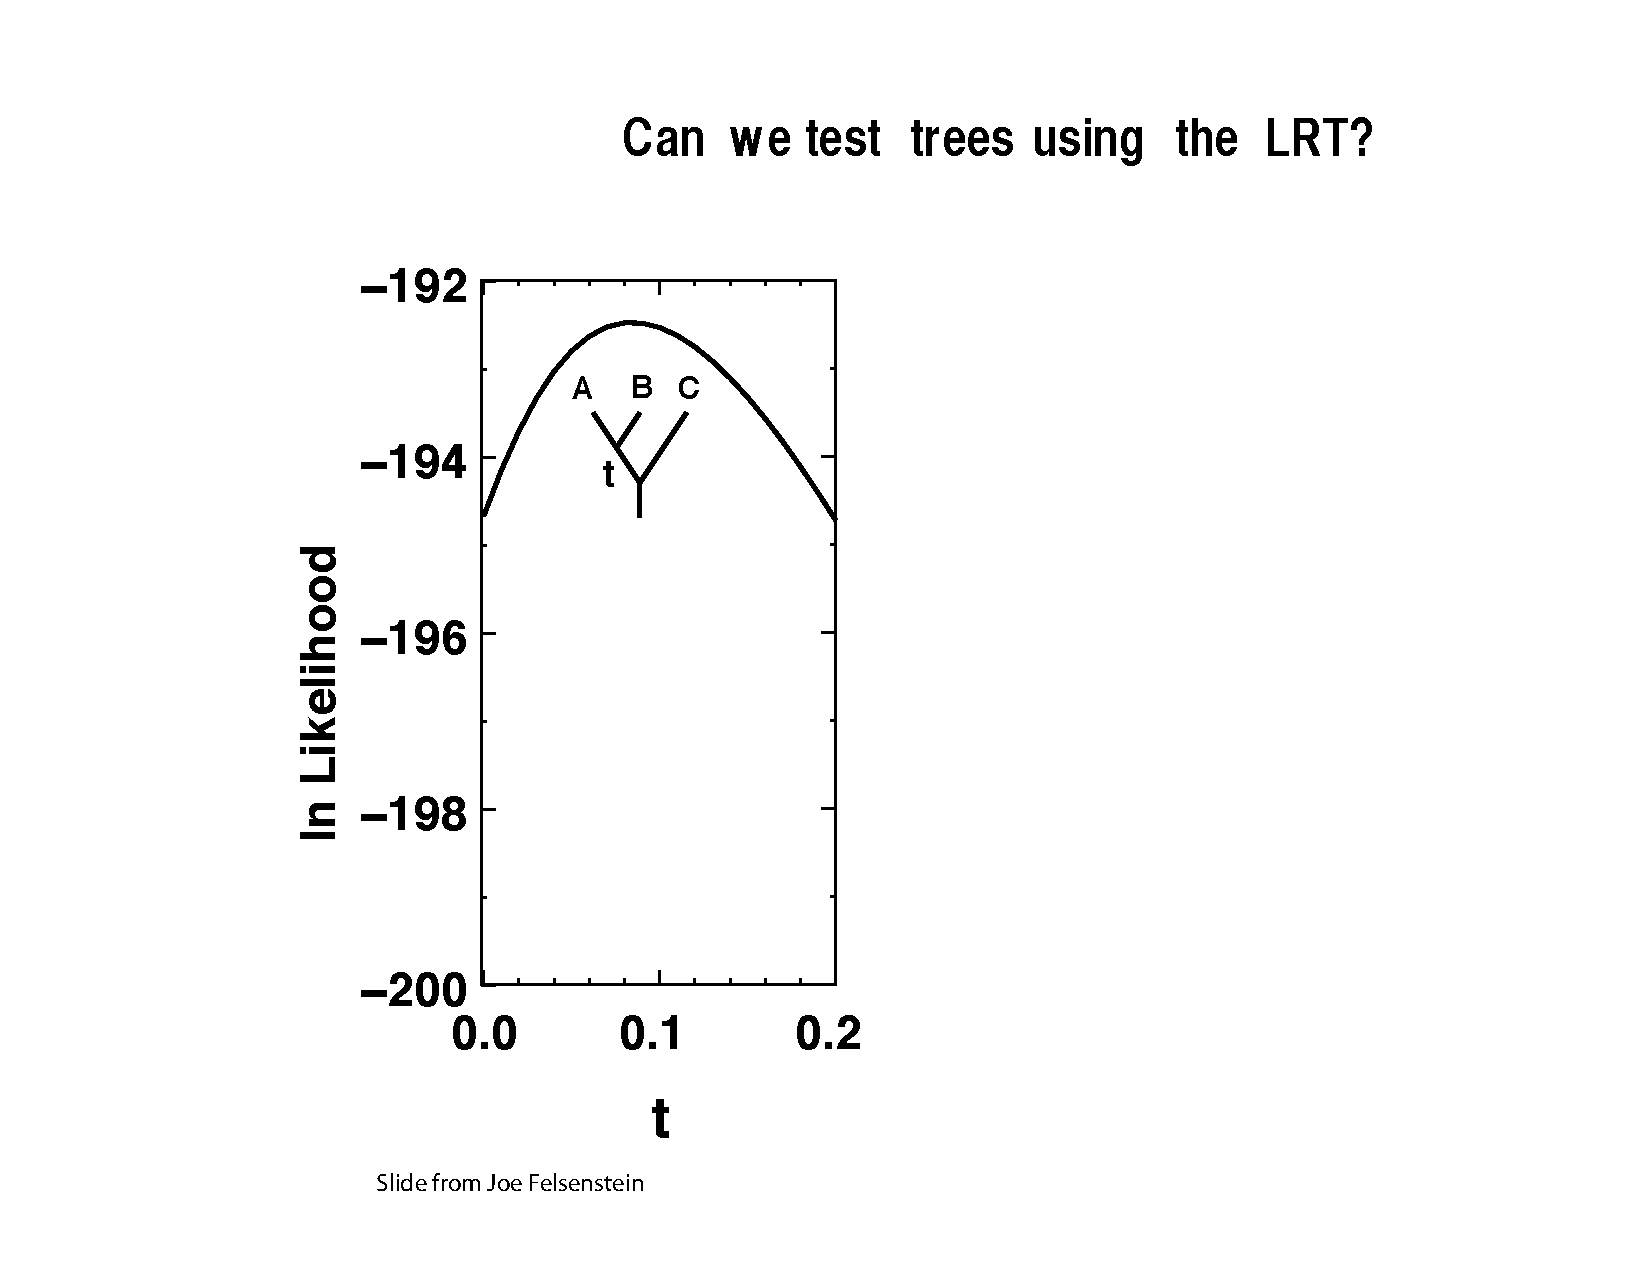
\includegraphics[scale=1.0]{../newimages/JoeFelsTreeLRT1.pdf}}}
	  \put(250,-100){1. Should we calculate the LRT as:}
	  \put(230,-140){$\delta_i = 2\left[\ln L(t=\hat{t},T_i|X) - \ln L(t=0,T_i|X)\right]$}
	  \put(250,-180){? }
	  \put(250,-250){2. And can we use the $\chi_1^2$ distribution to}
	  \put(250,-290){get the critical value for $\delta$?}
\end{picture}

\myNewSlide
\begin{picture}(500,0)(0,0)
	  \put(-200,-190){\makebox(0,0)[l]{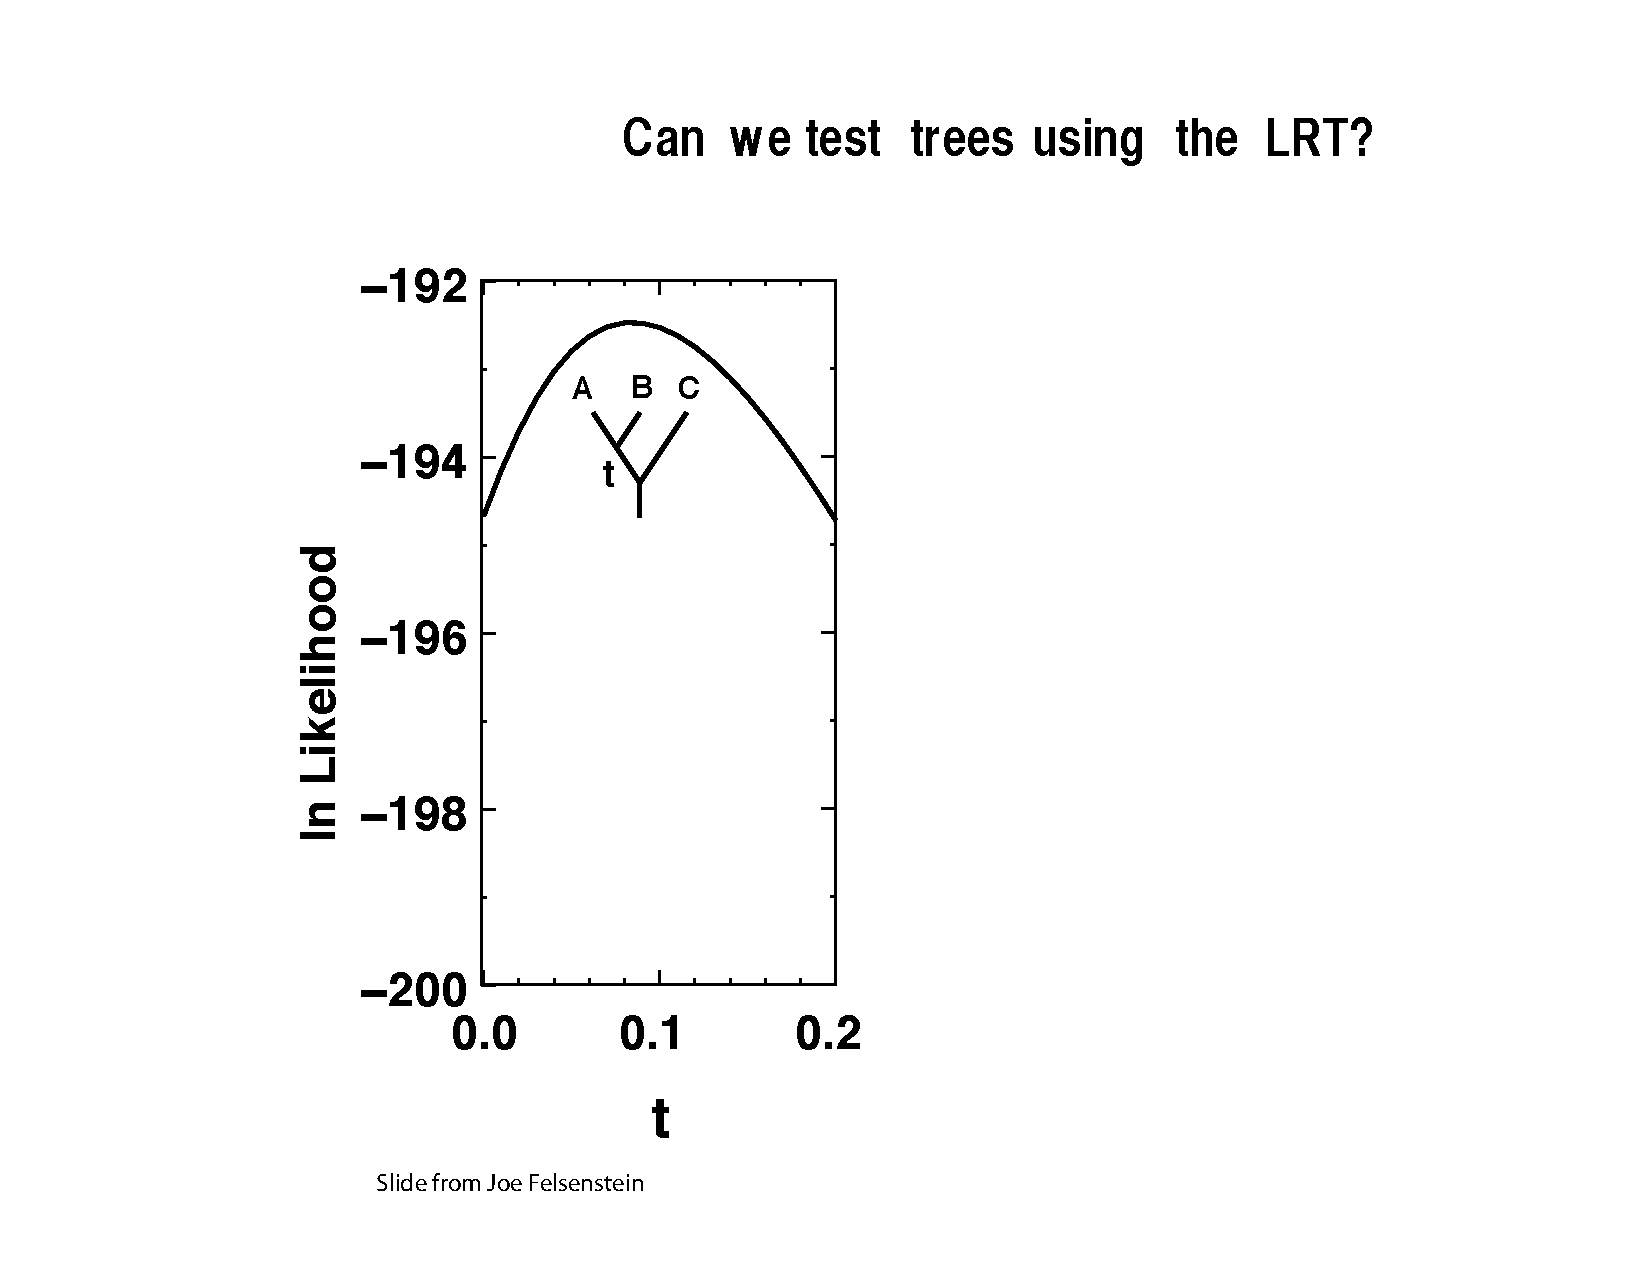
\includegraphics[scale=1.0]{../newimages/JoeFelsTreeLRT1.pdf}}}
	  \put(250,-100){1. Should we calculate the LRT as:}
	  \put(230,-140){$\delta_i = 2\left[\ln L(t=\hat{t},T_i|X) - \ln L(t=0,T_i|X)\right]$}
	  \put(250,-180){? {\bf \color{red}No. $t=0$ might not yield the best}}
	  \put(260,-220){\bf\color{red} alternative $\ln L$}
	  \put(250,-290){2. And can we use the $\chi_1^2$ distribution to}
	  \put(250,-330){get the critical value for $\delta$ ?}
	  \put(250,-370){{\bf \color{red}No. Constraining parameters}}
	  \put(260,-410){{\bf \color{red}at boundaries leads to a mixture}}
	  \put(260,-450){{\bf \color{red}such as: $\frac{1}{2}\chi_0^2 + \frac{1}{2}\chi_1^2$}}
	  \put(260,-490){\small See \citet{OtaWHSK2000}.}
\end{picture}

\myNewSlide
\begin{picture}(500,0)(0,0)
	  \put(-200,-190){\makebox(0,0)[l]{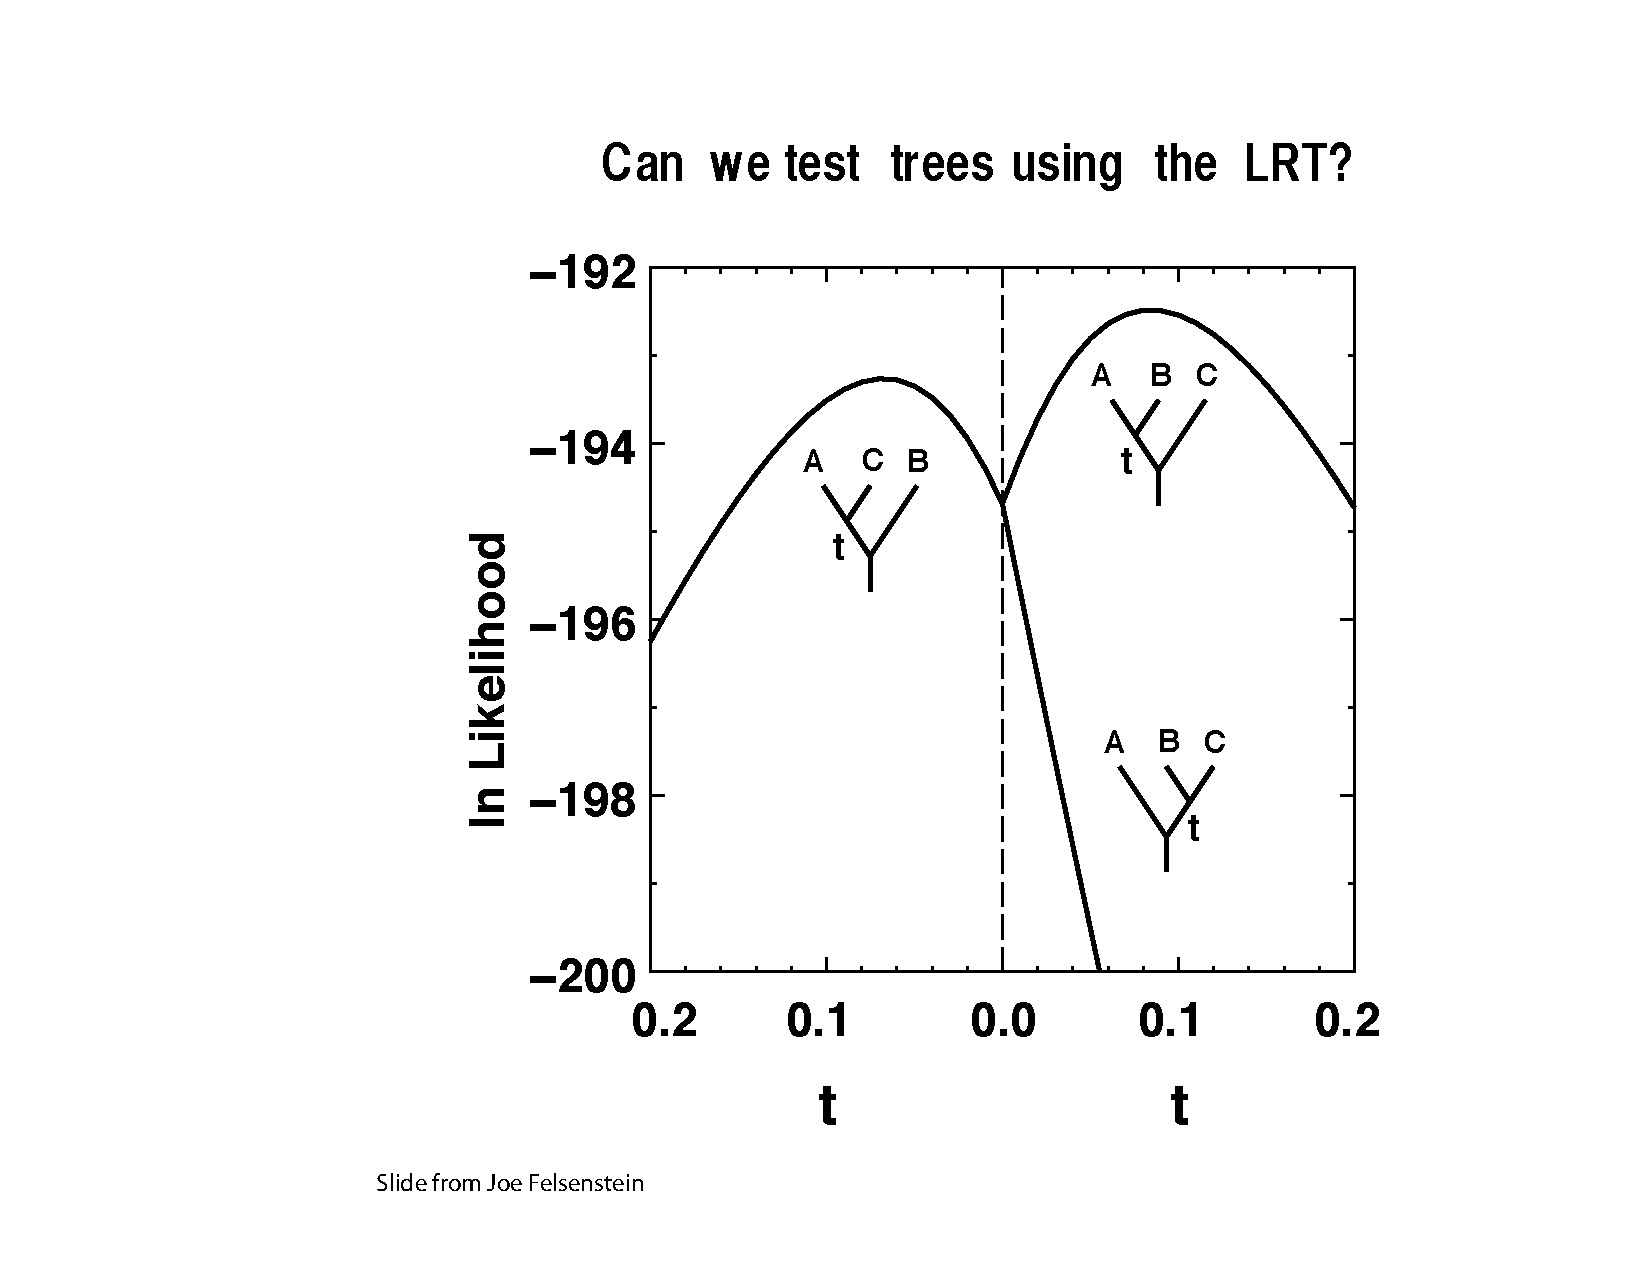
\includegraphics[scale=1.0]{../newimages/JoeFelsTreeLRT2.pdf}}}
\end{picture}

\myNewSlide
\section*{Parametric bootstrapping (and SOWH test)}
Generate the null distribution of $\delta_i$ by:
\begin{compactitem}
	\item finding the best tree and model pair that are consistent with the $H_0$,
	\item Simulating a large number $B$ of data sets, $X^{(1)}, X^{(2)},\ldots,X^{(B)}$ according to the parameters of that model,
	\item Calculating $\delta^{(j)} = 2\left[\ln L (\hat{T}; X^{(j)}) - \ln L (\hat{T}_{0}; X^{(j)})\right]$ where $\hat{T}_{0}$ is the tree estimated when you enforce a constraint such that all of the trees are compatible with the null.
\end{compactitem}

Intuitive and powerful, but not robust to model violation \citep{Buckley2002}.

\myNewSlide
\includepdf[pages={1-2}]{/Users/mholder/Documents/ku_teaching/BIOL-848-2010/images/gtr_i_g_sim_hist_data.pdf} 


\myNewSlide
\includepdf[pages={1-2}]{/Users/mholder/Documents/ku_teaching/BIOL-848-2010/images/jc_sim_hist_data.pdf} 

\myNewSlide
\section*{aLRT of \citet{AnisimovaG2006}}
\begin{compactitem}
	\item For a {\bf branch} $j$, calculate $\delta_{j}^{\dag}$ as twice the difference in $\ln L$ between the optimal tree (which has the branch) and the best NNI neighbor that lacks the branch.
	\item This is very fast, and can be done in PhyML.
	\item The argue that the null distribution for each LRT around the polytomy follows a $\frac{1}{2}\chi_0^2 + \frac{1}{2}\chi_1^2$ distribution
	\item The introduce Bonferroni-correction appropriate for correcting for the selection of the best of the three resolutions.
	\item They find aLRT to be accurate and powerful in simulations, but \citet{AnisimovaGDDG2011} report that it rejects too often and is sensitive to model violation.
\end{compactitem}
	
\myNewSlide
\section*{aBayes \citet{AnisimovaGDDG2011} }

For a branch of interest, $j$, Let's call the optimal tree that contains the branch $T_j$.
We'll call the 2 NNI neighbors of $T_j$  which lack $j$ ``$T_a$'' and ``$T_b$.''

$$\mbox{aBayes}(T_j|X) = \frac{\Pr(X|T_j)}{\Pr(X|T_j) + \Pr(X|T_a) + \Pr(X|T_b)}$$

Simulation studies of \citet{AnisimovaGDDG2011} show it to have the best power of the methods that do not have inflated probability of falsely rejecting the null.

It is sensitive to model violation



\myNewSlide
\normalsize
\bibliography{phylo}
\end{document}

\myNewSlide
\section*{Frequentist phylogenetic hypothesis testing?}
If we have a tree, $T_0$, in mind {\em a priori}, then how can we answer the question:

``Based on this data, should we reject the tree?'' 

Clearly if $\hat{T}\neq T_0$, then there is a possibility that we should reject $T$.  

But how do we calculate a p-value?

\myNewSlide
\section*{Frequentist phylogenetic hypothesis testing? (cont)}
What is our test-statistic? {\color{red} Difference in support between the null tree and the preferred tree.}

How do we find the null-distribution for the test statistic? {\color{red} Simulation}

\myNewSlide
\includepdf[pages={2}]{../lec14Testing/images/polBremer.pdf} 


\myNewSlide
\section*{Testing 2 trees}
\Large
Test statistic: The difference in score, $\delta$, between two trees chosen {\em a priori}.

Null hypothesis: Both trees are equally good explanations of the truth.

\[E(\delta) = 0\]

Is $\delta$ so large that we reject the null?\\ What if $\delta=-9$, should we reject the null?

\myNewSlide
\includepdf[pages={1}]{images/hivarsitediff.pdf} 

\myNewSlide
\includepdf[pages={1}]{images/lowvarsitediff.pdf} 

\myNewSlide
\section*{Tests that treat the number of variable length characters as fixed}
\large
\begin{compactenum}
	\item Winning sites test (test the null that there is an equal probability of a site favoring tree 1 over tree 2)
	\item Templeton's test a version of Wilcoxon's rank sum test
\end{compactenum}
Robust, but not very powerful

\myNewSlide
\includepdf[pages={1}]{images/hivardist.pdf} 

\myNewSlide
\includepdf[pages={1}]{images/lowvardist.pdf} 

\myNewSlide
I could generate the last 4 slides because I made up (and hence knew) a variance.

How can we assess the strength of support if we do not know the variance of the generating process?



\myNewSlide
\section*{Parametric bootstrapping}
\begin{compactenum}
	\item Simulate a large number of data sets on $T_0$. On each dataset, $i$:
	\begin{compactenum}
		\item Search for the preferred tree, $\hat{T}^{(i)}$
		\item Search for the best tree that is consistent with the null hypothesis, $T_0^{(i)}$
		\item Let $z_0^{(i)}$ be the difference in score  between these trees for data set $i$
	\end{compactenum}
	\item See if the observed test statistic $z$ is in the $\alpha$\% tail of the distribution $\mathbf{z}_0$
\end{compactenum}

\myNewSlide
\includepdf[pages={1-2}]{images/gtr_i_g_sim_hist_data.pdf} 

\myNewSlide
Parametric bootstrapping is powerful, but can also be sensitive to the model chosen to generate the data.

\myNewSlide
\includepdf[pages={1-2}]{images/jc_sim_hist_data.pdf} 


\myNewSlide
\section*{Kishino Hasegawa Test}
\begin{compactenum}
	\item Several variants:
	\begin{compactenum}
		\item parametric - using a normal approximation
		\item non-parametric - using a bootstrapping
	\end{compactenum}
	\item Appropriate for testing the null hypothesis that two trees explain the data equally well.
	\item {\bf Both} trees for the test must be specified from prior knowledge.
	\item Use the site-to-site variation in $\delta$ to estimate the variance of a Normal distribution
	\item In the null the mean is 0
\end{compactenum}

\myNewSlide
\includepdf[pages={8}]{images/polTopoTests.pdf} 

\myNewSlide
\section*{Kishino Hasegawa Test (bootstrapping)}
Rather than assume a Normal distribution and estimate a variance, it is common to bootstrap the
data to generate a null distribution of the total difference in score between 2 trees.

Bootstrapping is resampling your data to mimic the variability in the process that generated the data.


\myNewSlide
\includepdf[pages={33-34}]{images/joeTesting.pdf} 

\myNewSlide
\section*{Kishino Hasegawa Test (bootstrapping - continued)}
Bootstrapping can give us a sense of the variability, but if the original data favored tree 1 isn't it very likely that the bootstrapped replicates will be more likely to support tree 1 than tree 2?

This does not sound like we are following our null that both trees are equally good.

Solution: we must center the bootstrapped differences in score.
\myNewSlide
\includepdf[pages={2}]{images/polTopoTests.pdf} 

\myNewSlide
\includepdf[pages={4-5}]{images/polTopoTests.pdf} 

\myNewSlide
\includepdf[pages={10}]{images/polTopoTests.pdf} 

\myNewSlide
\includepdf[pages={4-7}]{images/polBoot.pdf} 
\end{document}     

\end{document}     

